\documentclass[10pt]{article}
\usepackage[a4paper,margin=1.5cm]{geometry}
\usepackage[utf8]{inputenc}
\usepackage{xurl}
\usepackage{seqsplit}

\usepackage[T1]{fontenc}
\usepackage[brazilian]{babel}
\usepackage{amsmath}
\usepackage{amssymb}
\usepackage{graphicx}
\usepackage{booktabs}
\usepackage{float}
\usepackage[hidelinks]{hyperref}
\setlength{\parskip}{2pt}
\setlength{\textfloatsep}{7pt}
\setlength{\intextsep}{7pt}
\newcommand{\code}[1]{\texttt{\seqsplit{#1}}}
\renewcommand{\refname}{Referências}
\renewcommand{\tablename}{Tabela}
\renewcommand{\figurename}{Figura}

\title{\vspace{-1.5cm}Meta-dataset e ranking de algoritmos}
\author{Carlos Henrique}
\date{}

\begin{document}
\maketitle
\vspace{-0.5cm}
\noindent\textbf{Código:} \url{https://github.com/carloshendvpm/projeto01-mtl}

\section{Descrição do meta-dataset e do problema}

Utilizei 30 datasets do repositório
\href{https://github.com/JusciAvelino/imbalancedRegression}{\texttt{imbalancedRegression}},
da profa. Juscimara Avelino, com 60 a 20\,640 instâncias e 5 a 320 preditores
numéricos, sem valores faltantes. A primeira coluna contém o alvo $y$.
As bases são: a1, a2, a3, a7, abalone, acceleration, airfoild,
analcatdata\_apnea3, available\_power, boston, california, cocomo\_numeric,
compactiv, concreteStrength, cpu\_small, debutanizer, forestFires,
fuel\_consumption\_country, heat, kdd\_coil\_1, lungcancer\_shedden,
maximal\_torque, meta, mortgage, pdgfr, sensory, space\_ga, treasury,
triazines e wine\_quality.

\textbf{Algoritmos e performances ($P$ e $R$).} Comparei
\code{LinearRegression}, \code{KNeighborsRegressor},
\code{DecisionTreeRegressor}, \code{RandomForestRegressor},
\code{GradientBoostingRegressor} e \code{SVR} do \code{scikit-learn},
com hiperparâmetros padrão e semente 42 nos modelos aleatórios.
Linear, KNN e SVR usaram \code{StandardScaler}, ajustado no treino de cada fold.

Escolhi SERA~\cite{sera} por sua relação com minha pesquisa em regressão
desbalanceada: a métrica incorpora a relevância $\varphi(y)$ aos erros
quadráticos, dando maior peso aos extremos. Menor SERA indica melhor desempenho.
Usei relevância automática por boxplot, com ambas as caudas, coeficiente
$1{,}5$ e integração de passo $0{,}01$, estimada no alvo de cada fold de teste.
O \texttt{KFold} teve 10 folds, embaralhamento e semente 42, com partições
iguais para todos os algoritmos. As médias das 1\,800 performances formam
$P\in\mathbb{R}^{30\times6}$; seus ranks por linha formam $R$, com posição 1
para o menor SERA e rank médio nos empates.

\textbf{Meta-características ($X$).} Cada dataset tem 13 descritores:
número de instâncias $n$ e preditores $p$; razão $n/p$; médias das médias,
desvios padrão, assimetrias e curtoses dos preditores; assimetria, curtose
e coeficiente de variação do alvo
($\operatorname{std}(y)/\operatorname{mean}(y)$, com desvio populacional);
e três descritores de relevância: \texttt{pct\_relevante}, dado por
$n^{-1}\sum_{i=1}^{n}\mathbf{1}\{\varphi(y_i)\geq0{,}8\}$, e sua decomposição
em \texttt{pct\_relevante\_alta} e \texttt{pct\_relevante\_baixa} (a mesma
soma, restrita a $y_i$ acima ou abaixo da mediana). Criei essa decomposição
porque \texttt{pct\_relevante} sozinho não distingue um dataset com extremos
só de um lado (ex.: airfoild, só cauda alta) de um com extremos nas duas
pontas (ex.: pdgfr, triazines); a maioria dos 30 datasets tem
\texttt{pct\_relevante\_baixa}$=0$. Nos três, a relevância é estimada no
dataset completo; o limiar $0{,}8$ define a proporção relevante, sem alterar
a SERA. Obtive $X\in\mathbb{R}^{30\times13}$, sem valores não finitos.

\textbf{Pergunta.} Para um novo dataset com alvos observados, aprender com
$X$ permite recomendar algoritmos com menor erro nos valores relevantes
do que usar um ranking fixo aprendido em outros datasets?

\textbf{Abordagens.} AR e MR re-ranqueiam a média e a mediana das colunas
de $R$, respectivamente. Vitórias significativas ordena o total de vitórias
nos 15 pares de algoritmos por dataset, usando Wilcoxon signed-rank
bilateral sobre os folds ($\alpha=0{,}05$); vence o menor SERA médio quando
$p<\alpha$. As Abordagens 1 e 2 usam \code{RandomForestRegressor}
multissaída para prever $P$ e $R$, respectivamente, com semente 42 e demais
hiperparâmetros padrão. As previsões são convertidas em ranks.

HARRIS~\cite{harris} usa 30 árvores, profundidade máxima 4, mínimo de 2
exemplos por folha, bootstrap e $\lfloor\sqrt{11}\rfloor=3$ atributos
candidatos por nó. Os splits minimizam a perda ponderada dos filhos,
$L=\lambda L_{\mathrm{ranking}}+(1-\lambda)L_{\text{regressão}}$.
A primeira componente é a média de $(1-\rho)/2$, com Spearman $\rho$
em relação ao consenso de Borda; a segunda é o erro quadrático médio
em relação à média do nó, com $P$ escalado pelo mínimo e máximo globais
do treino. A floresta calcula a média das performances preditas pelas
folhas e a converte em ranking.

\section{Resultados}

Usei \emph{leave-one-dataset-out}: em cada uma das 30 rodadas, treinei
as seis abordagens em 29 datasets e avaliei no restante. As agregações
e a escala de $P$ no HARRIS também usam apenas o treino.
Na comparação principal, fixei $\lambda=0{,}5$ (escolhido antes de rodar a
avaliação, para não favorecer a posteriori o valor que por acaso vencesse);
os cinco valores solicitados são apresentados separadamente.

Para a ordem recomendada $\pi_d$, defini a perda após $t$ testes e a
área discreta conforme o enunciado:
\[
 \ell_d(t)=\min_{1\leq j\leq t}P_{d,\pi_d(j)}-\min_a P_{d,a},
 \qquad A_d=\frac{1}{6}\sum_{t=1}^{6}\ell_d(t).
\]
Calculei as médias entre datasets na escala original e após dividir
$\ell_d(t)$ pela faixa $\max_a P_{d,a}-\min_a P_{d,a}$, com perda zero
para faixa nula. A normalização reduz o domínio de datasets como
california, cujo SERA fica entre $10^{12}$ e $10^{13}$.
Recuperei as perdas originais dos CSVs multiplicando as curvas
normalizadas pelas respectivas faixas antes de calcular as médias.

\begin{table}[H]
\centering\small
\begin{tabular}{lrrr}
\toprule
Abordagem & Spearman médio $\uparrow$ & Área original $\downarrow$ & Área normalizada $\downarrow$ \\
\midrule
HARRIS & $\mathbf{0{,}621}$ & $7{,}505\times 10^{9}$ & $0{,}039$ \\
AR & $0{,}616$ & $1{,}367\times 10^{6}$ & $0{,}038$ \\
Vitórias significativas & $0{,}616$ & $1{,}367\times 10^{6}$ & $0{,}038$ \\
Abordagem 2 & $0{,}609$ & $\mathbf{9{,}114\times 10^{5}}$ & $\mathbf{0{,}030}$ \\
MR & $0{,}605$ & $4{,}258\times 10^{9}$ & $0{,}051$ \\
Abordagem 1 & $0{,}543$ & $9{,}399\times 10^{5}$ & $0{,}046$ \\
\bottomrule
\end{tabular}
\caption{Resultados das seis abordagens nas 30 rodadas; HARRIS com $\lambda=0{,}5$.}
\label{tab:abordagens}
\end{table}

\begin{table}[H]
\centering\small
\begin{tabular}{rrrr}
\toprule
$\lambda$ & Spearman médio $\uparrow$ & Área original $\downarrow$ & Área normalizada $\downarrow$ \\
\midrule
$0{,}000$ & $0{,}560$ & $7{,}505\times 10^{9}$ & $0{,}046$ \\
$0{,}250$ & $0{,}585$ & $7{,}505\times 10^{9}$ & $0{,}048$ \\
$0{,}500$ & $0{,}621$ & $7{,}505\times 10^{9}$ & $0{,}039$ \\
$0{,}750$ & $0{,}615$ & $7{,}505\times 10^{9}$ & $0{,}039$ \\
$1{,}000$ & $0{,}623$ & $7{,}505\times 10^{9}$ & $0{,}040$ \\
\bottomrule
\end{tabular}
\caption{HARRIS: $\lambda=0$ usa somente perda de regressão nos splits;
$\lambda=1$, somente perda de ranking. Valores exibidos são arredondados.}
\label{tab:harris}
\end{table}

\begin{figure}[H]
\centering
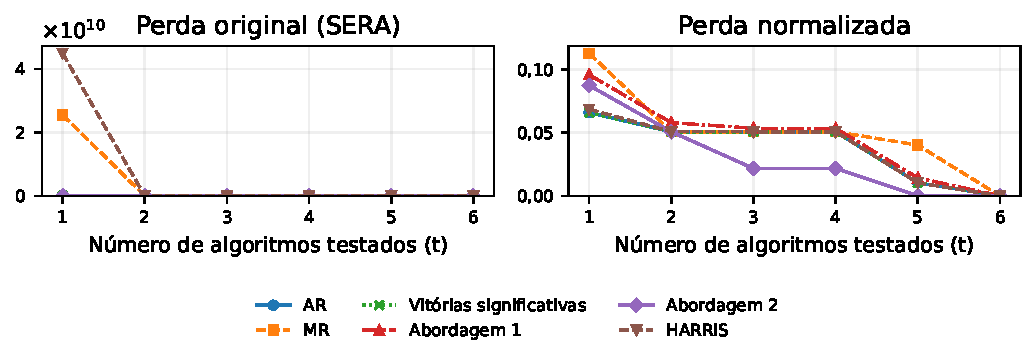
\includegraphics[width=\textwidth]{assets/relatorio/curvas_perda.pdf}
\caption{Curvas médias das seis abordagens. AR e Vitórias significativas
coincidem. Todas chegam a perda zero em $t=6$. Na escala original,
algumas curvas ficam visualmente próximas de zero.}
\label{fig:curvas}
\end{figure}

\textbf{Efeito do resampling.} O projeto acima mede o desbalanceamento
(via SERA e $\varphi$) mas não intervém nele. Para testar se intervir muda
a recomendação, gerei uma segunda matriz $P$ (mesmos 30 datasets, 10 folds,
seed e 6 algoritmos) reamostrando cada fold de treino com
WERCS~\cite{branco2019}. Escolhi WERCS, entre as estratégias do mesmo
repositório, porque usa a relevância $\varphi$ diretamente como peso
contínuo de inclusão/remoção, sem exigir um limiar (diferente de SMOGN,
\textit{random over/undersampling} e ruído gaussiano, que pedem
\code{rel\_thres}) -- reaproveitando a mesma $\varphi$ do SERA -- e por não
sintetizar instâncias novas, só duplicar/remover as existentes, reduzindo o
risco de erro de implementação. Usei os parâmetros padrão do pacote
(\code{over=0,5}, \code{under=0,5}, sem busca de hiperparâmetro). Comparei
o ranking resultante ($R_{\text{resampling}}$)
com o original ($R$): a correlação de Spearman entre os dois é $0{,}724$, e
o algoritmo de melhor rank muda em 19 dos 30 datasets ($63\%$) -- uma
mudança real, não ruído. No agregado (AR sobre cada matriz), RF e GB
permanecem nas duas primeiras posições nos dois cenários, mas SVR sobe do
$6^\circ$ para o $3^\circ$ lugar com resampling, e DT cai do $3^\circ$ para
o $5^\circ$:

\begin{table}[H]
\centering\small
\begin{tabular}{lrr}
\toprule
Algoritmo & AR sem resampling & AR com resampling \\
\midrule
RF & 1.0 & 1.0 \\
GB & 2.0 & 2.0 \\
DT & 3.0 & 5.0 \\
KNN & 4.0 & 4.0 \\
Linear & 5.0 & 6.0 \\
SVR & 6.0 & 3.0 \\
\bottomrule
\end{tabular}
\caption{AR (rank médio) calculado sobre $R$ e sobre $R_{\text{resampling}}$.}
\label{tab:resampling-ar}
\end{table}

Isso sugere que SVR se beneficia de reamostragem por relevância mais do que
DT nesses datasets -- hipótese não testada isoladamente aqui.

\section{Interpretação}

\textbf{Comparação estatística.} O teste de Friedman sobre o Spearman
por dataset não indicou diferença entre as seis abordagens:
$\chi^2(5)=3{,}4298$, $p=0{,}6340$. O Nemenyi~\cite{demsar}, incluído
conforme o enunciado, também não detectou diferenças a $\alpha=0{,}05$
(Figura~\ref{fig:cd}). Esses testes avaliam Spearman, não as áreas,
e não estabelecem equivalência. MR lidera o diagrama porque o eixo usa
ranks médios por dataset, enquanto a Tabela~\ref{tab:abordagens}
apresenta Spearman médio.

\begin{figure}[H]
\centering
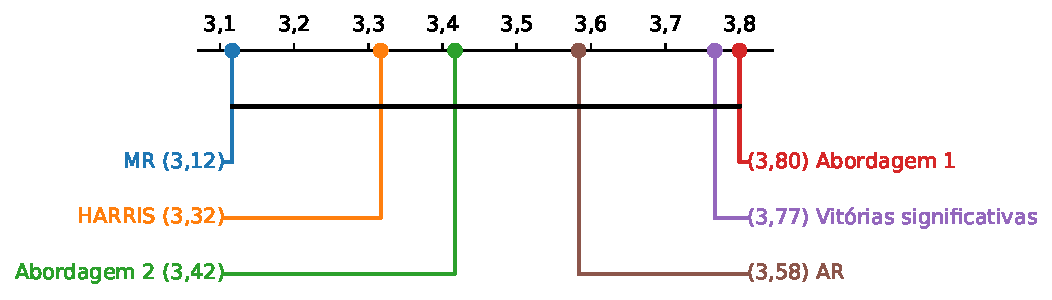
\includegraphics[width=0.85\textwidth]{assets/relatorio/diferenca_critica.pdf}
\caption{Diagrama de diferença crítica sobre Spearman, com Nemenyi a
$\alpha=0{,}05$. Menor rank médio é melhor; a barra conecta todas as
abordagens sem diferença detectada.}
\label{fig:cd}
\end{figure}

\textbf{Agregações versus aprendizado.} Nenhuma abordagem venceu nas duas
métricas ao mesmo tempo. No Spearman médio, HARRIS ($0{,}621$) superou AR
($0{,}616$) e a Abordagem 2 ($0{,}609$), mas cabeça-a-cabeça contra AR
ganhou em 5 datasets, perdeu em 2 e empatou em 23 -- a maioria empata
exatamente, comum com só 6 posições possíveis por ranking. Já na área
normalizada, a Abordagem 2 seguiu sendo a melhor ($0{,}030$, contra $0{,}038$
do AR e $0{,}039$ do HARRIS): Spearman pondera a ordem inteira, enquanto a
área pesa mais os primeiros testes. AR foi melhor em $t=1$ ($0{,}065943$ de
perda normalizada, contra $0{,}068620$ do HARRIS e $0{,}087449$ da Abordagem
2); em $t=2$ os três praticamente empatam ($\approx0{,}0508$), pois tendem
a colocar RF e GB nas duas primeiras posições, variando só a ordem entre
eles (Figura~\ref{fig:curvas}).

A Abordagem 1 teve o pior Spearman médio; MR, a pior área normalizada; e
HARRIS ($\lambda=0{,}5$), a pior área original. Prever $P$ bruto exige lidar
com escalas heterogêneas, enquanto $R$ é limitado a posições de 1 a 6 --
hipótese plausível para a diferença entre Abordagens 1 e 2, não uma causa
isolada experimentalmente.

\textbf{Efeito de $\lambda$.} O Spearman médio cresce de $0{,}560$
($\lambda=0$, só perda de regressão) até $0{,}623$ ($\lambda=1$, só perda
de ranking), com uma queda pontual em $\lambda=0{,}75$ ($0{,}615$) que
impede uma leitura estritamente monotônica; as áreas seguem o mesmo padrão
geral (Tabela~\ref{tab:harris}). É uma análise de sensibilidade sobre 5
valores fixados a priori, não uma busca de hiperparâmetro.

\textbf{Limitações.} Foram usados 30 datasets, sem análise de poder
estatístico. Com só 29 meta-instâncias de treino por rodada e 13
descritores, o espaço para aprender um padrão robusto é pequeno --
estrutural ao desenho, não corrigível sem mais datasets equivalentes; a
vantagem modesta e inconsistente de Abordagem 2/HARRIS sobre AR é
compatível com isso. O Wilcoxon por fold envolve treinos sobrepostos, e os
15 testes por dataset não tiveram correção por multiplicidade. Os empates
nas curvas seguem o \texttt{sort\_values}, sem avaliação de seu impacto. O
resampling usou só WERCS, parâmetros padrão -- vale só para essa
configuração, sem comparar com outras estratégias do mesmo repositório
(SMOGN, ruído gaussiano). O estudo cobre uma semente e as configurações
descritas; as versões das bibliotecas não foram registradas.

Os resultados não demonstraram vantagem geral de aprender com $X$
sobre as agregações. AR permaneceu competitivo, sobretudo quando
poucos algoritmos podem ser testados.

\begingroup
\small
\begin{thebibliography}{4}
\setlength{\itemsep}{0pt}
\bibitem{sera} Ribeiro, R. P.; Moniz, N. (2020).
\emph{Imbalanced regression and extreme value prediction}.
Machine Learning, 109, 1803--1835.
\href{https://doi.org/10.1007/s10994-020-05900-9}{doi:10.1007/s10994-020-05900-9}.
\bibitem{branco2019} Branco, P.; Torgo, L.; Ribeiro, R. P. (2019).
\emph{Pre-processing approaches for imbalanced distributions in regression}.
Neurocomputing, 343, 76--99.
\href{https://doi.org/10.1016/j.neucom.2018.11.100}{doi:10.1016/j.neucom.2018.11.100}.
\bibitem{harris} Fehring, L.; Hanselle, J.; Tornede, A. (2022).
\emph{HARRIS: Hybrid Ranking and Regression Forests for Algorithm Selection}.
\href{https://arxiv.org/abs/2210.17341}{arXiv:2210.17341}.
\bibitem{demsar} Demšar, J. (2006).
\emph{Statistical Comparisons of Classifiers over Multiple Data Sets}.
\href{https://www.jmlr.org/papers/v7/demsar06a.html}{JMLR, 7, 1--30}.
\end{thebibliography}
\endgroup
\end{document}
